\documentclass{llncs}

\usepackage{amsmath} % for equation*
\usepackage{wasysym} % for \Box
\usepackage{color}
\usepackage{hyperref}
\usepackage{graphicx}
\definecolor{darkgreen}{rgb}{0,0.7,0}

\newcommand{\myspace}[0]{\vspace*{0.25cm}}

% Fix link colors
\hypersetup{
  colorlinks = true,
  linkcolor=red,
  citecolor=red,
  urlcolor=blue,
  linktocpage % so that page numbers are clickable in toc
}


\newcommand{\answer}[1]{}%\color{red}\textit{#1}\color{black}}
\title{COMP 445 -- Theoretical Assignment 3 (TA3)\\ Winter 2018}

\author{Tristan Glatard\\
  \href{mailto:tristan.glatard@concordia.ca}{tristan.glatard@concordia.ca}
}

\institute{Concordia University\\
  Department of Computer Science and Software Engineering}

\begin{document}

\maketitle

\section*{Instructions}

\begin{itemize}
\item Please submit your assignment  as a pdf file on Moodle. The name of the pdf file must contain your name and student id. 
\item All questions will receive equal points.
\item Each question may have zero, one, or more than one
  correct choices.
\item Partial answers will receive partial marks only if no incorrect answer is selected.
\item Blank answers (no answer) will not be penalized.
\end{itemize}

\hrulefill\\

\myspace

\myspace

Student ID: \dotfill

\myspace

\myspace

First Name / Last Name: \dotfill

\myspace

\myspace

Signature: \dotfill

\myspace

\myspace

\hrulefill

\newpage

\section*{Network Layer}

\vfill
% Forwarding
\paragraph{\textbf{Q1:}}
To which interface will a datagram with destination IP address
132.205.221.134 (10000100 11001101 11011101 10000110 in binary) be
forwarded by a router with the following forwarding table? Assume that longest-prefix matching is used.

\begin{center}
\begin{tabular}{c|c}
  Destination address range & Link interface \\
  \hline
  10000100 11001101 11011101 ******** & 0\\
  \hline
  10000100 11001101 11011101 100***** & 1\\
  \hline
  10000100 11001101 11011101 10001*** & 2\\
  \hline
  Default  & 3
\end{tabular}
\end{center}

\begin{tabular}{ccl}
  a) & $\Box$ & 0\\
  \\
  b) & $\Box$ & 1\\
  \\
  c) & $\Box$ & 2\\
  \\
  d) & $\Box$ & 3\\
\end{tabular}

\vfill
% IPv4 header
\paragraph{\textbf{Q2:}}

The checksum of an IPv4 datagram header must be recomputed by \emph{every} router that forwards the datagram because:\\
\begin{tabular}{ccl}
  a) & $\Box$ & The destination IP address of the datagram changes in every router.\\
  \\
  b) & $\Box$ & The TTL (time-to-live) value of the datagram changes in every router.\\
  \\
  c) & $\Box$ & The upper layer field of the datagram changes in every router.\\
  \\
  d) & $\Box$ & The data in the datagram changes in every router.\\  
\end{tabular}

\vfill
% IP address
\paragraph{\textbf{Q3:}}
What is the subnet address associated with IP address 132.205.221.134/26?

\begin{tabular}{ccl}
  a) & $\Box$ & 132.205.0.0\\
  \\
  b) & $\Box$ & 132.205.221.0\\
  \\
  c) & $\Box$ & 132.205.221.128\\
  \\
  d) & $\Box$ & 132.205.221.134\\
\end{tabular}


% NAT table
\newpage
\vfill
\paragraph{\textbf{Q4:}}
Assuming the following NAT table in a router, to which private IP address and port will an incoming datagram with destination address 132.205.221.134 and port 4003 be translated?

\begin{center}
\begin{tabular}{c|c}
  WAN-side addr & LAN-side addr \\
  \hline
  132.205.221.134, 4001 & 10.0.0.1, 3421 \\
  132.205.221.134, 4002 & 10.0.0.1, 5431 \\
  132.205.221.134, 4003 & 10.0.0.2, 6722 \\
  132.205.221.134, 4004 & 10.0.0.3, 1234
\end{tabular}
\end{center}

\begin{tabular}{ccl}
  a) & $\Box$ &  132.205.221.134, 4001\\
  \\
  b) & $\Box$ &  132.205.221.134, 4002\\
  \\
  c) & $\Box$ &  10.0.0.2, 6722\\
  \\
  d) & $\Box$ &  10.0.0.3, 1234\\
\end{tabular}

\vfill
% IPv6
\paragraph{\textbf{Q5:}}
Version 6 of the ICMP protocol introduced a ``Packet Too Big'' error message because:

\begin{tabular}{ccl}
  a) & $\Box$ & The total datagram length might exceed the maximum transmission unit (MTU) of some networks.\\
  \\
  b) & $\Box$ & IPv6 does not support fragmentation.\\
  \\
  c) & $\Box$ & IPv6 does not have a header checksum.\\
  \\
  d) & $\Box$ & IPv6 might be tunneled in IPv4.\\
\end{tabular}
\vfill

\newpage
\paragraph{\textbf{Q6:}}
The content below was captured using
Wireshark:\\
\includegraphics[width=\textwidth]{ip.png}
This trace contains:\\
\begin{tabular}{ccl}
  a) & $\Box$ & An IPv6 datagram.\\
  \\
  b) & $\Box$ & An echo reply ICMP message.\\
  \\
  c) & $\Box$ & A TCP acknowledgment.\\
  \\
  d) & $\Box$ & An ICMP message encapsulated in an IP datagram.\\
\end{tabular}


% Dijkstra
\newpage
\paragraph{\textbf{Q7}:}
Considering the following network and table representing the first iteration of the Dijkstra algorithm to compute the least-cost paths from A, what will be the result of the second iteration of the Dijkstra algorithm?

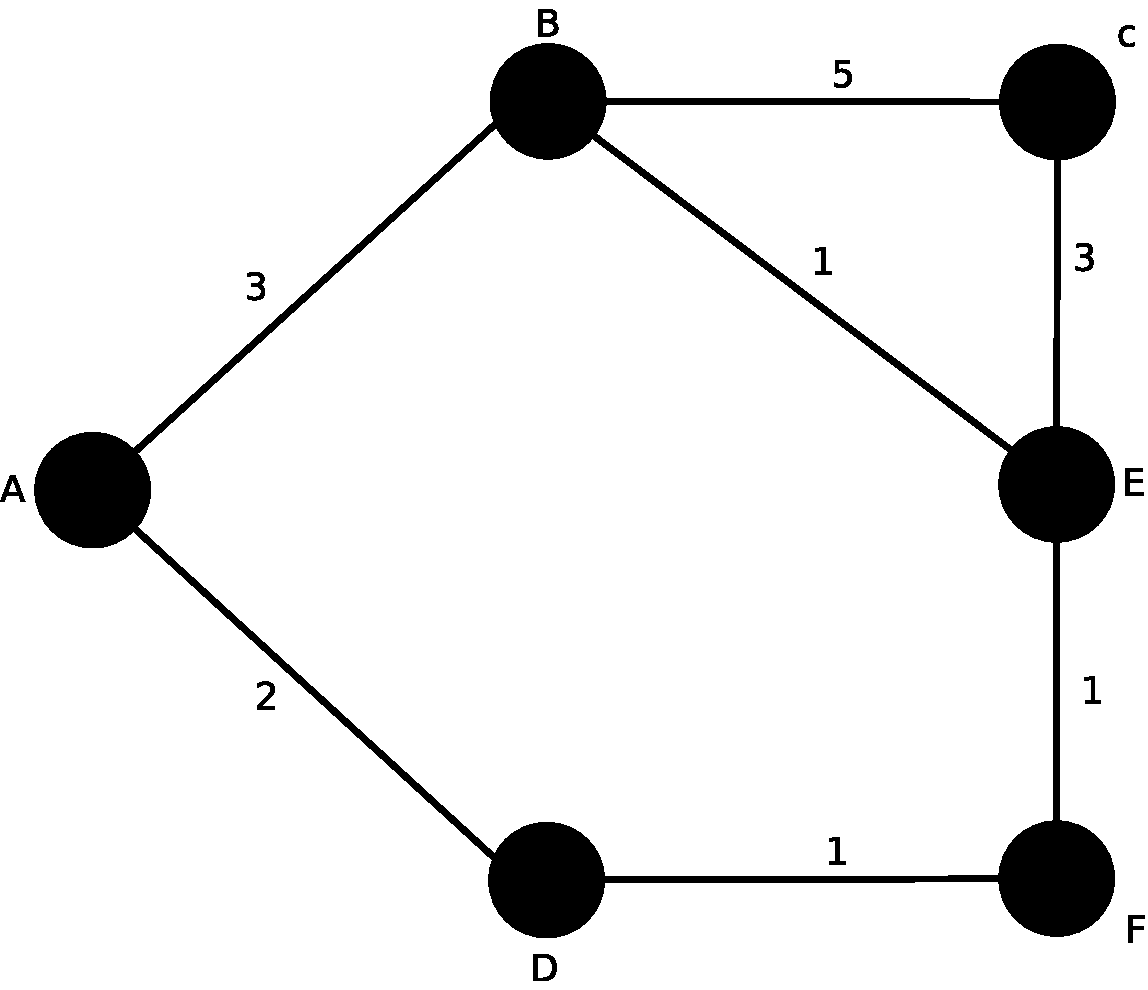
\includegraphics[width=0.5\textwidth]{graph.pdf}

First iteration of Dijkstra algorithm:\\
\begin{center}
    \begin{tabular}{l|c|c|c|c|c}
      N'     & B   & C        & D     & E        & F        \\
      \hline
      A      & 3,A & $\infty$ & 2,A   & $\infty$ & $\infty$ \\
    \end{tabular}
    \end{center}

    Second iteration:\\
    \vspace*{0.3cm}
    
\begin{tabular}{ccl}
  a) & $\Box$ &     \begin{tabular}{l|c|c|c|c|c}
      N'     & B   & C        & D     & E        & F        \\
      \hline
      A      & 3,A & $\infty$ & 2,A   & $\infty$ & $\infty$ \\
      AB     &     & 8,B & 2,A   & 4,B & $\infty$ \\
    \end{tabular}
  \\
  \\
  b) & $\Box$ &     \begin{tabular}{l|c|c|c|c|c}
      N'     & B   & C        & D     & E        & F        \\
      \hline
      A      & 3,A & $\infty$ & 2,A   & $\infty$ & $\infty$ \\
      AD & 3,A & $\infty$ &      & $\infty$ & 3,D \\
    \end{tabular}
\\
  \\
  c) & $\Box$ & \begin{tabular}{l|c|c|c|c|c}
      N'     & B   & C        & D     & E        & F        \\
      \hline
      A      & 3,A & $\infty$ & 2,A   & $\infty$ & $\infty$ \\
      AC & 3,A & 8,B & 2,A & 4,B & $\infty$\\
    \end{tabular}\\
  \\
  d) & $\Box$ & \begin{tabular}{l|c|c|c|c|c}
      N'     & B   & C        & D     & E        & F        \\
      \hline
      A      & 3,A & $\infty$ & 2,A   & $\infty$ & $\infty$ \\
      AE & 3,A & 7,E & 2,A & 4,B & 5,E
    \end{tabular}\\
\end{tabular}

\newpage
% DV
\paragraph{\textbf{Q8}:}

Considering the following Distance-Vector table in node X, of the network below, what would be the updated table in node X after X received the following notification from node Z?\\

\begin{center}
  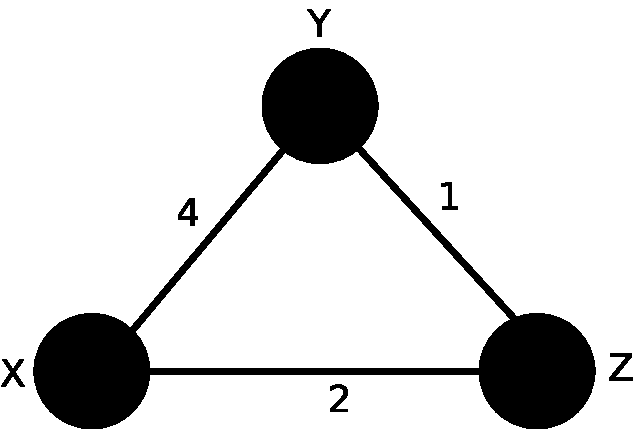
\includegraphics[width=0.3\textwidth]{graph1.pdf}
\end{center}

Initial table in node X:
\begin{center}
\begin{tabular}{c|c|c|c}
  & X & Y & Z \\
  \hline
  X & 0 & 4 & 2 \\
  Y & $\infty$ & $\infty$ & $\infty$\\
  Z & $\infty$ & $\infty$ & $\infty$\\
\end{tabular}
\end{center}

Notification received from node Z:
\begin{center}
\begin{tabular}{c|c|c|c}
  & X & Y & Z \\
  \hline
  Z & 2 & 1 & 0 \\
\end{tabular}
\end{center}

Updated table in X:\\
\begin{tabular}{ccl}
  a) & $\Box$ &  \begin{tabular}{c|c|c|c}
    & X & Y & Z \\
    \hline
    X & 0 & 4 & 2 \\
    Y & $\infty$ & $\infty$ & $\infty$\\
    Z & 2 & 1 & 0 \\
  \end{tabular}\\
  \\
  b) & $\Box$ & \begin{tabular}{c|c|c|c}
    & X & Y & Z \\
    \hline
    X & 0 & 3 & 2 \\
    Y & $\infty$ & $\infty$ & $\infty$\\
    Z & 2 & 1 & 0 \\
  \end{tabular}\\
  \\
  c) & $\Box$ & \begin{tabular}{c|c|c|c}
    & X & Y & Z \\
    \hline
    X & 0 & 3 & 2 \\
    Y & 3 & 0 & 1 \\
    Z & 2 & 1 & 0 \\
  \end{tabular}\\
  \\
  d) & $\Box$ &    \begin{tabular}{c|c|c|c}
    & X & Y & Z \\
    \hline
    X & 0 & 4 & 2 \\
    Y & $\infty$ & $\infty$ & $\infty$\\
    Z & $\infty$ & $\infty$ & $\infty$\\
  \end{tabular}
\end{tabular}

% BGP
%\paragraph{\textbf{Q8:  }}

\newpage
\section*{Link Layer}

\vfill
\paragraph{\textbf{Q9}:}
Among the addresses below, which one(s) represent a MAC address?

\begin{tabular}{ccl}
  a) & $\Box$ & 132.205.221.134\\
  \\
  b) & $\Box$ & fe80::7bd6:63dd:dccb:2cda\\
  \\
  c) & $\Box$ & 00:0e:c6:e2:05:f3\\
  \\
  d) & $\Box$ & www.concordia.ca\\
\end{tabular}

\vfill
\paragraph{\textbf{Q10:}}
Assuming the following table in a switch with 4 interfaces numbered
from 0 to 3, to which interface would a frame with destination
00:0e:c6:e2:05:f3 be forwarded?

\vspace*{0.3cm}
\begin{center}
\begin{tabular}{c|c}
  MAC addr & Interface \\
  \hline
  02:42:fa:0d:f7:0d & 0 \\
  52:54:00:b3:1a:d5 & 0 \\
  f0:d5:bf:50:80:98 & 1 \\
\end{tabular}
\vspace*{0.3cm}
\end{center}

\begin{tabular}{ccl}
  a) & $\Box$ & 0\\
  \\
  b) & $\Box$ & 1\\
  \\
  c) & $\Box$ & 2\\
  \\
  d) & $\Box$ & 3\\
\end{tabular}
\vfill

\end{document}
